
\chapter{Premesse sulla paginazione}
La paginazione è l'argomento che storicamente confonde di più gli studenti. Si tenga conto che l'argomento sarà affrontato anche nel corso di \textit{Sistemi Operativi}.
\section{Recap con prime questioni}
\begin{itemize}
	\item \textbf{Memory mapped I/O}. 
	
	Lo spazio di indirizzamento include la RAM (che occupa una minima parte dello spazio), ma anche periferiche come APIC, memoria video in modalità testo, memoria video in modalità grafica. La cosa ci ha creato problemi relativamente alle periferiche \emph{memory mapped}: la cache deve essere disattivata, non può memorizzare cacheline relativamente ad istruzioni di I/O. L'unica cosa che possiamo fare è distinguere le operazioni a partire dagli indirizzi.
	\item \textbf{Protezione}. 
	
	Abbiamo diviso la memoria RAM in due parti: la parte $M1$ per il sistema e la parte $M2$ per l'utente. I meccanismi di protezione fanno sì che l'utente non possa accedere in alcun modo alla prima area di memoria (nè operazioni di lettura, nè di scrittura).  Abbiamo dei problemi relativi all'\textbf{isolamento tra processi}. La protezione agisce anche sulle istruzioni di un programma: posso leggerle ma non modificarle. Inoltre, viene vietato l'utilizzo dell'indirizzo $0$, poiché \emph{nullptr} (anche in modalità sistema).
	\item \textbf{Multiprogrammazione}. 
	
	Abbiamo anche detto che ogni volta che attraversiamo il gate ed effettuiamo un cambio di processo dobbiamo memorizzare il \emph{contesto}. Il contesto non si limita ai soli registri, ma anche al contenuto della memoria. Se vogliamo fare i precisi diventa necessario spostare l'intera area di memoria nell'hard disk (cioè in qualcosa di più grande). Questa cosa funziona molto bene con memorie RAM piccole, ma adesso è problematica (oggi fare uno spostamento del genere significa lavorare con diversi GB).
\end{itemize} 
\clearpage 
\section{Idea di base: tenere insieme informazioni di più processi} Abbiamo bisogno di un meccanismo che minimizzi gli spostamenti tra RAM e hard disk, limitandoci al minimo indispensabile. L'idea è tenere in memoria RAM le informazioni relative a più processi, cioè trattare la RAM come una sorta di cache dell'hard disk. Si considerino le seguenti problematiche.
\begin{itemize}
	\item \textbf{Dimensione massima di ogni processo} 
	
	La prima cosa che dobbiamo chiederci è di quanto spazio ha bisogno ogni processo. Dobbiamo tenere conto delle seguenti aree:
	\begin{itemize}
		\item \emph{text} (codice programma) e \emph{data} (variabili globali), dimensione nota al collegatore e costante per tutta l'esecuzione del programma;
		\item pila e \emph{heap}, aree di memoria (inizialmente vuote) che possono espandersi durante l'esecuzione del programma.
	\end{itemize}
	L'area di memoria di un processo è organizzata così
	\begin{center}
		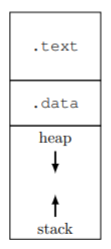
\includegraphics{img/208.PNG}
	\end{center}
	\emph{heap} e pila stanno in un'area unica, con direzioni di espansione opposte.  
	
	\noindent \textbf{Soluzione}. Quello che faremo è porre dimensione massima per l'area dedicata a \emph{heap} e pila. Solitamente si pone un valore di default. 
	
	\item \textbf{Isolamento tra i processi}	
	
	Abbiamo detto che l'idea base è mettere insieme, nella RAM, più processi. Senza il ricorso al meccanismo della protezione il processo in esecuzione potrebbe intervenire sullo stato dei processi non in esecuzione.
	
	\noindent \textbf{Soluzione}. L'idea risolutiva potrebbe essere l'aggiunta di due nuovi registri nella CPU: LINF (limite inferiore) ed LSUP (limite superiore). Segue l'inserimento di questi due registri nel \emph{contesto} in \emph{des$\_$proc}. \begin{itemize} 
		\item Chiaramente i due registri sono scrivibili solo a livello sistema.
		\item Se ci troviamo a livello utente la CPU controlla che ogni accesso memoria sia compreso tra LINF ed LSUP, altrimenti lancia un'eccezione.
		\item Ogni volta che un processo viene caricato dall'hard disk il sistema deve inizializzare gli appositi campi \emph{contesto} con l'indirizzo finale e iniziale della parte di memoria occupata dal processo.
		\item Ogni volta che si cambia processo si aggiorna il contenuto di LINF ed LSUP nel processore, prendendo come valori quelli relativi al processo entrante.
	\end{itemize}  
	Attenzione: questa soluzione non è quella definitiva (quando introdurremo la paginazione vedremo perchè non servono questi registri).
	
	\item \textbf{Caricamento a indirizzi variabili}
	
	L'indirizzo dove andiamo a caricare il processo non è più chiaro come prima: il processo può essere caricato ovunque e la sua posizione dipende anche dagli altri processi posti nella RAM. L'indirizzo dove carichiamo il processo non è quindi noto durante compilazione e collegamento.
	\begin{itemize}
		\item \textbf{Grosso problema}. Se io rimuovo un processo e lo metto in un punto diverso della memoria gli indirizzi relativi al processo non sono più validi, dovrei correggerli rispetto alla nuova posizione: questa cosa non è possibile, poichè gli indirizzi sono indistinguibili.
		\item \textbf{Soluzione}. La soluzione è utilizzare il registro LINF come indirizzo di base. L'indirizzo $x$ in un processo è diverso dall'indirizzo $x$ in un altro processo: nel programma ci limitiamo a indicare l'offset, che si somma a LINF per ottenere l'indirizzo vero e proprio a cui puntare. 
	\end{itemize}
	Attenzione: questa soluzione non è quella definitiva (quando introdurremo la paginazione vedremo perchè non serve il registro LINF e come facciamo a ricondurci al cosiddetto \emph{indirizzo fisico}).
\end{itemize}
\section{Step successivo: memoria virtuale e indirizzi virtuali}
Riflettiamo un po' di più sull'ultima questione affrontata: quella degli indirizzi variabili. Fino ad oggi abbiamo utilizzato solo ed esclusivamente i cosiddetti \textbf{indirizzi fisici}. Adesso introduciamo gli \textbf{indirizzi virtuali} e la \emph{memoria virtuale}.
\begin{itemize}
	\item \underline{Il codice del programma relativo a un processo utilizza esclusivamente \emph{indirizzi virtuali}}.
	\item Questi \emph{indirizzi virtuali} sono relativi al processo, cioè l'indirizzo $x$ di un presunto processo $P1$ non sarà uguale all'indirizzo $x$ di un processo $P2$.
	\item Se consideriamo la soluzione provvisoria per gli indirizzi otteniamo quello fisico così
	\[\text{Indirizzo fisico}=\text{LINF}+\text{Indirizzo virtuale}\]
\end{itemize}

\paragraph{Cioè?} Dobbiamo distinguere lo \emph{spazio di indirizzamento fisico} (dove troviamo RAM e qualunque periferica) dallo \emph{spazio di indirizzamento virtuale}. I processi non hanno alcun accesso allo spazio di indirizzamento fisico: vedono solo lo spazio di indirizzamento virtuale, che è una sorta di mondo immaginario dove troviamo la \emph{memoria virtuale}. In questa memoria sono presenti le solite parti: \emph{text}, \emph{data}, \emph{heap} e \emph{stack}.
\begin{center}
	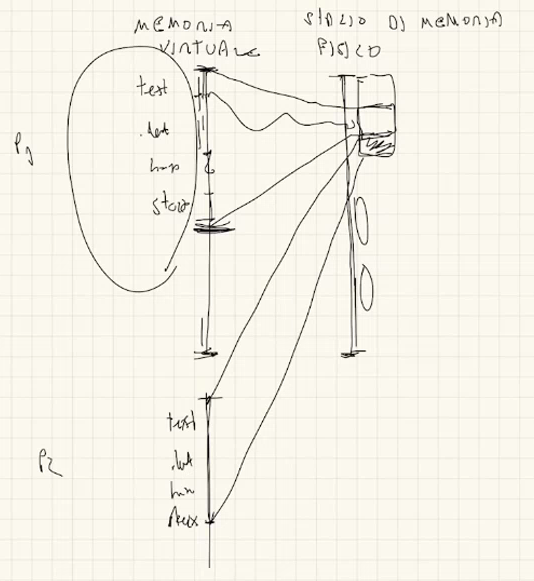
\includegraphics[scale=.65]{img/209.PNG}
\end{center} 
L'hardware, attraverso una unità che vedremo più avanti, trasforma gli indirizzi di \emph{text}, \emph{data}, \emph{heap} e \emph{stack} in indirizzi dello spazio di memoria fisico (\textit{un po' come i film Western dove di una casa c'è solo la facciata}, cit.).
\subsection{Scopo del Kernel} Quello che avremo è una situazione dove il programma si interfaccia con una CPU e una RAM virtuali.
\begin{itemize}
	\item La CPU è il contesto che abbiamo salvato nel descrittore di processo, che verrà caricato nella CPU vera (si aggiorna lo stato della CPU fisica in divisione di tempo, ma si rappresenta lo stato della CPU virtuale).
	\item La memoria RAM non viene gestita in divisione di tempo (come ipotizzato all'inizio), ma in divisione di spazio: la RAM contiene, in contemporanea, più immagini di processi diversi.
\end{itemize} 
Tutte queste cose sono affrontate dal \emph{kernel}.

\paragraph{Definizione di \emph{kernel} su Wikipedia} \textit{Un kernel, in informatica costituisce il nucleo o core di un sistema operativo, ovvero il software che fornisce un accesso sicuro e controllato dell'hardware ai processi in esecuzione sul computer. Dato che possono eventualmente esserne eseguiti simultaneamente più di uno, il kernel può avere anche la responsabilità di assegnare una porzione di tempo-macchina (scheduling) e di accesso all'hardware a ciascun programma (multitasking)}.

\clearpage 

\section{Tutto finito?}

Il meccanismo di cui abbiamo parlato fino ad ora presenta due svantaggi:
\begin{enumerate}
	\item Come possiamo condividere parte della memoria tra due o più processi?
	\item Cosa succede se dobbiamo caricare un processo, ma lo spazio in memoria è frammentato in porzioni troppo piccole? Questo problema potrebbe essere risolto
	\begin{enumerate}
		\item ricompattando lo spazio (ma questo significherebbe copiare un'intera porzione di memoria da una zona a un'altra), oppure
		\item spezzare la memoria di un processo in più porzioni e gestire ciascuna di queste separatamente.
	\end{enumerate}
\end{enumerate}
La soluzione (b) è la più interessante, visto che permette di risolvere anche il primo problema. 
\begin{center}
	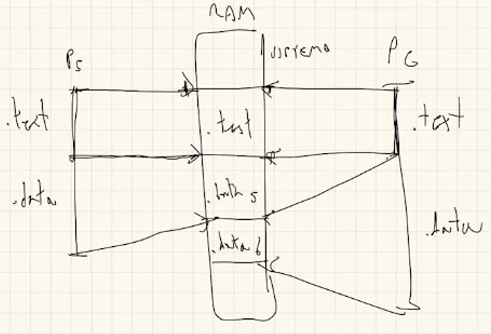
\includegraphics[scale=.8]{img/211.PNG}
\end{center} Tutto questo ci porta a parlare della \textbf{paginazione}, dove parti diverse dello spazio di indirizzamento di un processo si traducono in modo diverso (il passaggio da indirizzi virtuali a indirizzi fisici).